\section{Durchführung}
\label{sec:Durchführung}

\subsection{Wheatstone Brücke}
\begin{figure}[H]
    \centering
        \centering
        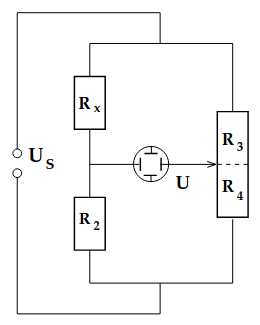
\includegraphics[width=0.35\textwidth]{Bilder/wheatstone.png}
        \caption{Wheatstone Brücke. \cite{anleitung}}
    \hfill
    \label{fig:f2}
\end{figure}


\subsection{Kapazitätsmessbrücke}
\begin{figure}[H]
    \centering
        \centering
        \includegraphics[width=0.35\textwidth]{Bilder/kapazitätsmess.png}
        \caption{Wheatstone Brücke. \cite{anleitung}}
    \hfill
    \label{fig:f3}
\end{figure}

\subsection{Induktivitätsmessbrücke}
\begin{figure}[H]
    \centering
        \centering
        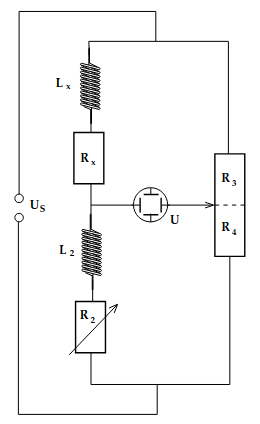
\includegraphics[width=0.35\textwidth]{Bilder/induktivitaetsmess.png}
        \caption{Wheatstone Brücke. \cite{anleitung}}
    \hfill
    \label{fig:f4}
\end{figure}

\subsection{Wien-Robinson Messbrücke}
\begin{figure}[H]
    \centering
        \centering
        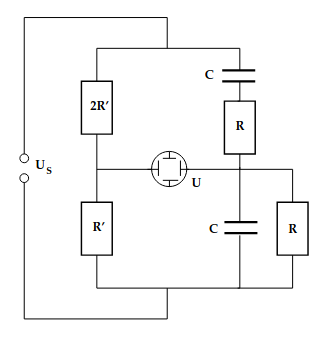
\includegraphics[width=0.35\textwidth]{Bilder/wien_robinson.png}
        \caption{Wheatstone Brücke. \cite{anleitung}}
    \hfill
    \label{fig:f5}
\end{figure}
